% Jacob Neumann

% DOCUMENT CLASS AND PACKAGE USE
\documentclass[aspectratio=169]{beamer}
 
% Establish the colorlambda boolean, to control whether the lambda is solid color (true), or the same as the picture (false)
\newif\ifcolorlambda
\colorlambdafalse % DEFAULT: false

% Use auxcolor for syntax highlighting
\newif\ifuseaux
\useauxfalse % DEFAULT: false

% Color settings
\useauxtrue

\newcommand{\auxColor}{008a25}     % the color of note boxes and stuff
\newcommand{\presentColor}{1FAB89} % the primary color of the slide borders
\newcommand{\bgColor}{f5fff5}      % the color of the background of the slide
\newcommand{\darkBg}{8b98ad}
\newcommand{\lambdaColor}{\auxColor}

\colorlambdatrue

\usepackage{comment} % comment blocks
\usepackage{soul} % strikethrough
\usepackage{listings} % code
\usepackage{makecell}

\setbeamertemplate{itemize items}[circle]
% \setbeameroption{show notes on second screen=right}

\usepackage{lectureSlides}
%%%%%%%%%%%%%%%%%%%%%%%%%%%%%%%%%%%%%%%%%| <----- Don't make the title any longer than this
\title{Structural Induction and Tail Recursion} % TODO
\subtitle{Inducting over exotic structures} % TODO
\date{25 May 2023} % TODO
\author{Brandon Wu} % TODO

\graphicspath{ {./img/} }
% DONT FORGET TO PUT [fragile] on frames with codeblocks, specs, etc.
    %\begin{frame}[fragile]
    %\begin{codeblock}
    %fun fact 0 = 1
    %  | fact n = n * fact(n-1)
    %\end{codeblock}
    %\end{frame}

% INCLUDING codefile:
    % 1. In some file under code/NN (where NN is the lecture id num), include:
%       (* FRAGMENT KK *)
%           <CONTENT>
%       (* END KK *)

%    Remember to not put anything on the same line as the FRAGMENT or END comment, as that won't be included. KK here is some (not-zero-padded) integer. Note that you MUST have fragments 0,1,...,KK-1 defined in this manner in order for fragment KK to be properly extracted.
    %  2. On the slide where you want code fragment K
            % \smlFrag[color]{KK}
    %     where 'color' is some color string (defaults to 'white'. Don't use presentColor.
%  3. If you want to offset the line numbers (e.g. have them start at line 5 instead of 1), use
            % \smlFragOffset[color]{KK}{5}

\begin{document}

% Make it so ./mkWeb works correctly
\ifweb
\renewcommand{\pause}{}
\fi

\setbeamertemplate{itemize items}[circle]

% SOLID COLOR TITLE (see SETTINGS.sty)
{
\begin{frame}[plain]
\colorlambdatrue
\titlepage
\end{frame}
}

\begin{frame}[fragile]
\frametitle{Lesson Plan}

\tableofcontents
\end{frame}

\begin{frame}[fragile]
  \frametitle{Last time}

  In the last lecture, we learned about the relationship between recursion 
  and induction. 

  \pause
  \vspace{\fill}
  
  We learned about some more fundamental constructs to the Standard ML language, such
  \term{case} and \code{let} expressions. 
  
  \pause
  \vspace{\fill}

  We then used these concepts to write an implementation of the \code{pow} function
  using naive recursion, as well as a faster variant \code{fast_pow}, using
  repeated squaring to do less work. 
\end{frame}

\sectionSlide{1}{Deconstructing Data}

\begin{frame}[fragile]
  \frametitle{What's in a List?}

  In the last lecture, we saw a brief treatment of lists and \code{case}
  expressions, which allow us to \term{deconstruct} lists, or dispatch
  on the kind of data that is present within a list. 

  \pause
  \vspace{\fill}

  We had an idea about how to think about lists, which is worth repeating now:

  \pause
  \vspace{5pt}

  \customBox{Mantra}{\, Lists can be either \code{[]} or \code{x::xs}, and
  \textit{nothing more}.}

  \pause
  \vspace{\fill}

  But what does that really mean? It means that doing anything that involves
  examining a list involves \textit{at least} two cases:

  \begin{codeblock}
    case L of
      [] => (* ... *)
    | x::xs => (* ... *) 
  \end{codeblock}
\end{frame}

\begin{frame}[fragile]
  \frametitle{What's in a List?}

  We can view this another way, equivalently: 

  \pause
  \vspace{\fill}

  \customBox{Mantra}{\, Lists can be either empty or not, and
  \textit{nothing more}.}

  \pause
  \vspace{\fill}

  But this perspective actually is significantly less useful for
  us. There is a slight distinction here.
\end{frame}

\begin{frame}[fragile]
  \frametitle{A List Problem}

  Suppose we are interested in writing the following list function:
  \spec
    {take}
    {int * int list -> int list}
    {\code{n >= 0}}
    {\code{take (n, L)} evaluates to the first \code{n} elements of \code{L}, 
    in order. If there are not enough elements, then \code{L} should just be
    however many elements are left.} 

\end{frame}

\begin{frame}[fragile]
  \frametitle{Some List Helpers}

  Recall our \code{isEmpty} function from before:
  \begin{codeblock}
    fun isEmpty (L : int list) : bool = 
      case L of
        [] => true
      | _ => false 
  \end{codeblock}

  \pause
  \vspace{\fill}

  We could also define a \code{hd} function, which takes off the
  first element of a list:
  \spec
    {hd}
    {int list -> int}
    {\code{L} is nonempty}
    {\code{hd L} evaluates to the first element of \code{L}}
  \pause
  \begin{codeblock}
    fun hd (x::xs : int list) : int = x 
      | hd [] = raise Fail "impossible"
  \end{codeblock}

\end{frame}

\begin{frame}[fragile]
  \frametitle{Some List Helpers}

  Furthermore, suppose we had a \code{tl} function, which takes
  every element but the first of a list: 
  \spec
    {tl}
    {int list -> int list}
    {\code{L} is nonempty}
    {\code{tl L} evaluates to \code{L}, excluding the first element}
  \pause
  \begin{codeblock}
    fun tl (x::xs : int list) : int list = xs 
      | tl [] = raise Fail "impossible"
  \end{codeblock}

  \pause
  \vspace{\fill}

  We'll use these to write our \code{take} function.
\end{frame}


\begin{frame}[fragile]
  \frametitle{\code{take}ing an \code{L}}

  \begin{codeblock}
    fun take (n : int, L : int list) : int list = 
      if isEmpty L orelse n = 0 then
        []
      else
        let
          val x = hd L 
          val xs = tl L 
        in
          x :: take (n - 1, xs)
        end
  \end{codeblock}

  \pause
  \vspace{\fill}

  What's wrong here?
\end{frame}

\begin{frame}[fragile]
  \frametitle{\code{take}ing an \code{L}}

  We see in this implementation of \code{take} that we are too reliant
  upon preconditions.

  \pause
  \vspace{\fill}

  \code{hd} and \code{tl} are functions which can possibly raise exceptions,
  so we have to be very careful about using them! In this case, we know that
  it is safe because of the \code{isEmpty} call, but this can quickly lead
  us to error if we are not careful.

  \pause
  \vspace{\fill}

  Moreover, it's wasteful! We pattern match once to get out a value of type
  \code{bool}, about whether or not the list is empty or not, and then we
  pattern match once more to get the head and tail out. \textbf{This is duplicated
  work!}
\end{frame}

\begin{frame}[fragile]
  \frametitle{Schrodinger's List}

  The issue is that we are adhering too much to the mantra that "a list is
  either empty or not empty". 

  \pause
  \vspace{\fill}

  This is a true statement, but it's strictly less powerful than the statement
  that a list is \code{[]} or \code{x::xs}. The former is a statement that only
  gives two kinds of information -- true or false. The second one sums up
  \textit{exactly what data is present in a list}. 

  \pause
  \vspace{\fill}

  This is another way of saying that pattern matching is strictly more powerful
  than \code{if} expressions.
\end{frame}

\begin{frame}[fragile]
  \frametitle{Parse, Don't Validate}

  This general idea is an instance of a popular idea in functional programming
  called "parse, don't validate".

  \pause
  \vspace{\fill}

  \defBox{}{\, We say that a function \code{p : t -> bool}, for some type
  \code{t}, is a \term{validator}. It ascertains some property $P$ of the
  input, and returns a boolean.}

  \pause
  \vspace{\fill}

  The idea is to avoid simply \term{validating} input by only producing a single
  value of truth because, as we saw with the \code{hd} and \code{tl} 
  example, this doesn't stop us from maybe having to query that property many times 
  down the road, producing wasted effort, and uglier code. 

  \pause
  \vspace{\fill}

  \defBox{}{\, We say that a function \code{f : t -> t2} is, in a sense,
  a \term{parser}\footnotemark, as opposed to a validator \code{p}, if it produces output data 
  such that the property \code{p} validates is present in the type of \code{t2}. 
  }

  \footnotetext[1]{This idea comes from 
  {\color{blue}\href{https://lexi-lambda.github.io/blog/2019/11/05/parse-don-t-validate/}{this excellent article}}.
  I should also disclaim that this is a nontraditional usage of the word "parse", so
  while you can apply this thinking, be careful in using this wording, as people
  might be confused what you mean.
  }
\end{frame}

\begin{frame}[fragile]
  \frametitle{\code{take} Two}

  Let's try rewriting \code{take} again, using this logic.

  \pause
  \begin{codeblock}
    fun take (n : int, L : int list) : int list =
      case (n, L) of
        (0, _)     => []
      | (_, [])    => []
      | (_, x::xs) => x :: take (n - 1, xs)
  \end{codeblock}

  \pause
  \vspace{\fill}

  \textbf{This code is much cleaner}. It avoids needing to use the \code{hd} and
  \code{tl} functions, which are possibly error-producing, and acts as a
  \term{parser}, because instead of using an intermediary \code{bool} as the
  signal for whether \code{L} is nonempty, in the nonempty case, it produces
  a value of type \code{int * int list}. 
\end{frame}

\begin{frame}[fragile]
  \frametitle{Types, Not Preconditions}

  \tgs

  The basic idea is that a value of type \code{int * int list} is more useful than
  a boolean, because \textbf{it itself is proof that the list 
  is nonempty}. A list which contains an \code{int} cannot be empty, and having
  access to the elements that are inside the list is strictly more powerful/useful.

  \pause
  \vspace{\fill}

  This is why pattern matching is more powerful than conditionals. It lets you see
  what values \textit{really are}, rather than simply querying them. It actually
  \textbf{produces the goods}, as opposed to just making claims.

  \pause
  \vspace{\fill}

  Viewed another way, "parse, don't validate" is about lifting preconditions to
  types instead of checks, wherever possible.
\end{frame}


\begin{frame}[fragile]
  \frametitle{Booleans are Weak}

  For example, let's take an example of some code that exhibits
  significant branching behavior:

  \pause
  \vspace{\fill}

  \begin{codeblock}
    if isEmpty L then
      (* 1 *) 
    else if List.length L >= 2 then
      (* 2 *)
    else if List.length L = 1 then
      if hd L = 2 then
        (* 3 *) 
      else
        (* 4 *)
  \end{codeblock}

\end{frame}
\begin{frame}[fragile]
  \frametitle{Pattern Matching is Overpowered}

  \begin{codeblock}
    case L of
      [] => (* 1 *)
    | x::y::xs => (* 2 *)
    | 2::xs => (* 3 *)
    | x::xs => (* 4 *)
  \end{codeblock}

  \pause
  \vspace{\fill}

  Much better.
\end{frame}

\sectionSlide{2}{Structural Induction}

\begin{frame}[fragile]
  \frametitle{Induction, another way}

  The induction principle on natural numbers lets us prove things about numbers by
  viewing them as \textit{built up from other numbers}. In essence, we are expanding our
  store of numbers for which we know the theorem to be true.

  \pause
  \vspace{\fill}

  By way of analogy, we might imagine a bucket.

  \pause
  \begin{figure} 
    \centering
    \includegraphics[scale=0.2]{bucket_empty} 
    \caption{Figure 1: The "Bucket of Mathematical Truth"\footnotemark}
  \end{figure}
  \pause
  This bucket is meant to contain all the things that we know satisfy our theorem-to-prove.
  \footnotetext[2]{Patent pending.}
\end{frame}

\begin{frame}[fragile]
  \frametitle{Induction, another way}

  By default, the bucket is empty. Our first action as theorem provers is to throw our base case
  into the bucket. In the case of induction on the natural numbers, this is zero.

  \pause
  \vspace{\fill}
  
  \begin{center} 
    \includegraphics[scale=0.3]{bucket_0} 
  \end{center}

  \pause
  \vspace{\fill}

  The bucket still has a ways to go, however! To prove our statement for the next number, 1, we
  will apply our \textit{inductive step}. 
\end{frame}

\begin{frame}[fragile]
  \frametitle{Induction, another way}

  This tells us that, from $P(0)$, we can achieve $P(1)$.

  \pause
  \vspace{\fill}

  \begin{center} \includegraphics[scale=0.3]{bucket_0_and_1} \end{center}
\end{frame}

\begin{frame}[fragile]
  \frametitle{Induction, another way}

  By analogy, you should be able to convince yourself that eventually, we can throw every single
  natural number into the bucket.

  \pause
  \begin{center} \includegraphics[scale=0.3]{bucket_n} \end{center}

  This means that, for any natural number $n$, we can \textit{eventually}, in finitely many
  applications of this logic, prove $P(n)$.

  \pause
  \vspace{\fill}

  This is the "bucket" view of mathematical induction.
\end{frame}

\begin{frame}[fragile]
  \frametitle{Induction Is Not Just For Cookware}

  In the last lecture, we learned about the \code{list} type constructor, which allows us
  to talk about types like \code{int list} and \code{string list}.

  \pause
  \vspace{\fill}

  Lists are not just good for storing data, but they admit a simple structure which allows 
  us to easily prove things about lists. For instance, consider the following function:

  \pause
  \begin{codeblock}
    fun length ([] : int list) : int = 0
      | length (x::xs) = 1 + length xs
  \end{codeblock}

  How might we convince ourselves that the \code{length} function is total?

  \pause
  \vspace{\fill}

  Recall that a function \code{f : t1 -> t2} is total if, for all values \code{v : t1}, there exists a
  \code{v' : t2} such that \code{f v} $\hookrightarrow$ \code{v'}. In other words, the function 
  reduces to a value for each valuable input.
\end{frame}

\begin{frame}[fragile]
  \frametitle{An Informal Proof}

  Intuitively, it seems like we could reason about the function like so:

  \pause
  \vspace{\fill}

  Clearly, the function \code{length} must terminate, because when given any list, 
  it must be either empty or have a first element. If it's the first case, then we 
  terminate, because \code{length} will return \code{0}. If not, then we will recurse
  and enter a shorter case, which is always guaranteed to enter a smaller case, which
  will eventually reach \code{[]}. 

  \pause
  \vspace{\fill}

  This is what is called a \term{paragraph proof}. 
\end{frame}

\begin{frame}[fragile]
  \frametitle{An Informal Proof}

  We would prefer to see formal proofs of correctness! Intuitive reasoning and 
  colloquial wording can mask errors, and precision is necessary when reasoning 
  about complex programs.

  \pause
  \vspace{\fill}

  Similarly to how we will avoid "dot dot dot" reasoning when proving claims 
  on the natural numbers, by using the technique of \term{mathematical induction},
  we will employ the technique of \term{structural induction} when proving claims
  about lists.
\end{frame}

\begin{frame}[fragile]
  \frametitle{Structural Induction on Lists}

  \ptmt

  \defBox{\, The principle of \term{structural induction on lists} is as follows:}

  \pause
  \vspace{\fill}

  Let $P$ be a theorem on values \code{v : t list}, for some type \code{t}. We would
  like to show that, for all values \code{v : t list}, $P(\code{v})$ holds.

  \pause
  \vspace{\fill}

  It suffices to show that:
  \begin{itemize}
    \item $P(\code{[]})$ holds
    \item Assuming that $P(\code{xs})$ holds, for some \code{xs : int list}, show that
    $P(\code{x::xs})$ holds, for an arbitrary \code{x : int}.
  \end{itemize}

  \pause
  \vspace{\fill}

  We call this \term{proof by structural induction}.
\end{frame}

\begin{frame}[fragile]
  \frametitle{Totally Total}

  \thmBox{}\, \code{length} is total
  
  \pause
  \vspace{\fill}

  We proceed by \term{structural induction} on \code{L : int list}.

  \pause
  \vspace{\fill}

  \bcBox{\, \code{L = []}}
  \begin{align*}
    \code{length []} &\eeq 0 & \text{(def. of \code{length})}
  \end{align*}
  \ihBox{}{\, Case: \code{L = xs}, for some \code{xs : int list}. Assume that \code{length xs} $\hookrightarrow$ \code{v}.}

  \isBox{}{\, Case: \code{L = x::xs}, for some \code{x : int}. Let's show that \code{length (x::xs)} $\hookrightarrow$ \code{v}.}
  \begin{align*}
    \code{length (x::xs)} &\stepsTo \code{1 + length xs} & \text{(clause 2 of \code{length})} \\
                          &\stepsTo^* \code{1 + v}         & \text{(inductive hypothesis)} \\
                          &\stepsTo \code{v'}            & \text{(totality of \code{+})}
  \end{align*}
\end{frame}

\begin{frame}[fragile]
  \frametitle{Buckets of Fun}

  The principle of structural induction on lists looks very similar to that of mathematical
  induction on the natural numbers!

  \pause
  \vspace{\fill}

  It's key to remember that the principle is just the same, in terms of what is "really happening"
  with the proof. We are showing that, through finite applications of the same inductive step,
  we can prove the claim for any list, from the empty list.

  \pause
  \vspace{\fill}

  To visualize this, our bucket for structural induction would start with just the empty list in it:

  \pause
  \begin{center} \includegraphics[scale=0.25]{bucket_nil} \end{center}
\end{frame}

\begin{frame}[fragile]
  \frametitle{Buckets of Fun}

  \rprs

  Upon the first application of the inductive step, we would then throw in \code{x::[]}, for any 
  \code{x : int}. Our bucket would then contain the empty list, along with every singleton 
  list.

  \pause
  \begin{center} \includegraphics[scale=0.3]{bucket_singletons} \end{center}

  \pause
  \vspace{\fill}

  Repeated application of this technique will eventually produce every single list of integers. 
\end{frame}

\begin{frame}[fragile]
  \frametitle{A Picture of Induction}
  
  \makebox[\textwidth][c]{
    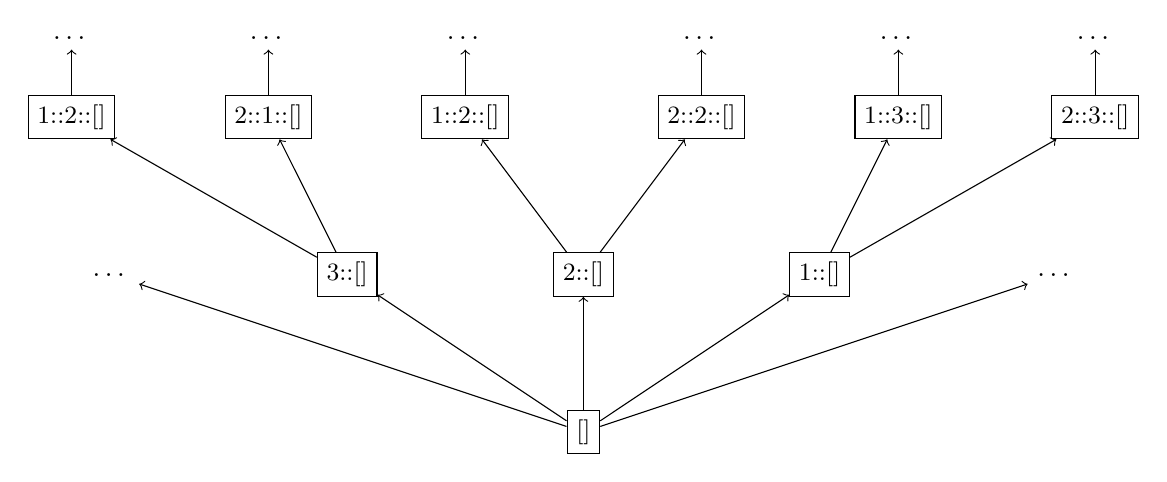
\begin{tikzpicture}
      \node[] (E1) at (-4.5,5) {\textellipsis};
      \node[shape=rectangle,draw=black] (T1) at (-4.5,4) {\small \code{1::2::[]}};

      \node[] (E2) at (-2,5) {\textellipsis};
      \node[shape=rectangle,draw=black] (T2) at (-2,4) {\small \code{2::1::[]}};

      \node[] (E3) at (0.5,5) {\textellipsis};
      \node[shape=rectangle,draw=black] (T3) at (0.5,4) {\small \code{1::2::[]}};

      \node[] (E4) at (3.5,5) {\textellipsis};
      \node[shape=rectangle,draw=black] (T4) at (3.5,4) {\small \code{2::2::[]}};

      \node[] (E5) at (6,5) {\textellipsis};
      \node[shape=rectangle,draw=black] (T5) at (6,4) {\small \code{1::3::[]}};

      \node[] (E6) at (8.5,5) {\textellipsis};
      \node[shape=rectangle,draw=black] (T6) at (8.5,4) {\small \code{2::3::[]}};

      \node[] (EL) at (-4,2) {\textellipsis};
      \node[shape=rectangle,draw=black] (M1) at (-1,2) {\small \code{3::[]}};
      \node[shape=rectangle,draw=black] (M2) at (2,2) {\small \code{2::[]}};
      \node[shape=rectangle,draw=black] (M3) at (5,2) {\small \code{1::[]}};
      \node[] (ER) at (8,2) {\textellipsis};

      \node[shape=rectangle,draw=black] (L) at (2,0) {\small \code{[]}} ;

      \draw[<-] (E1) -- (T1);
      \draw[<-] (E2) -- (T2);
      \draw[<-] (E3) -- (T3);
      \draw[<-] (E4) -- (T4);
      \draw[<-] (E5) -- (T5);
      \draw[<-] (E6) -- (T6);

      \draw[<-] (T1) -- (M1);
      \draw[<-] (T2) -- (M1);
      \draw[<-] (T3) -- (M2);
      \draw[<-] (T4) -- (M2);
      \draw[<-] (T5) -- (M3);
      \draw[<-] (T6) -- (M3);

      \draw[<-] (EL) -- (L);
      \draw[<-] (M1) -- (L);
      \draw[<-] (M2) -- (L);
      \draw[<-] (M3) -- (L);
      \draw[<-] (ER) -- (L);
  \end{tikzpicture}
  }

  \vspace{\fill}

  Every node represents a particular value at which our theorem needs to hold,
  and the edges depict applications of the inductive step \code{x::xs}, at 
  different values of \code{x}.
\end{frame}


\begin{frame}[fragile]
  \frametitle{Quantity is Quality}

  One thing to be wary of is to be sure you have correct quantification in your inductive proof.

  \pause
  \vspace{\fill}

  A surefire way to lose points on a homework is to write the following statement:

  "Assume that, for all \code{xs : int list}, $P(\code{xs})$ holds"

  \pause
  Why? This is assuming the theorem!

  \pause
  \vspace{\fill}

  Technically, the structural induction principle for lists looks like:
  $$P(\code{[]}) \land (\forall \code{xs}, \code{x}:[P(\code{xs}) \implies P(\code{x::xs})]) \implies (\forall \code{L} : [P(\code{L})])\footnotemark$$

  \pause
  We do not assume that $P(\code{xs})$ holds for all \code{xs}, we show that for all \code{xs}, 
  if $P(\code{xs})$ holds, then we also have $P(\code{x::xs})$!

  \pause
  \vspace{\fill}

  It is best to be safe and explicit in your proofs by writing the case out explicitly, as well as what variables
  you are introducing for it.

  \footnotetext[3]{Where \code{x, xs, L} range over values such that \code{x : int}, \code{xs : int list}, and \code{L : int list}}
\end{frame}

\begin{frame}[fragile]
  \frametitle{A Template for Induction on Lists}

  We proceed by structural induction on \code{L : int list}.

  \vspace{\fill}

  \bcBox{\, Case: \code{L = []}} 

  \vspace{5pt}

  $\langle$ proof that $P(\code{[]})$ holds $\rangle$

  \vspace{\fill}

  \ihBox{}{\, Case: \code{L = xs}}. Assume that the theorem holds for \code{xs}. 

  \vspace{5pt}

  \isBox{}{\, Case: \code{L = x::xs}}. We would like to show that $P(\code{x::xs})$ holds. 

  \vspace{5pt}
  
  $\langle$ proof of $P(\code{x::xs})$, under hypothesis that $P(\code{xs})$ holds $\rangle$

  \vspace{\fill}

  Thus, by the principle of structural induction, the theorem holds for all \code{L}.
\end{frame}

\sectionSlide{3}{Tail Recursion}

\begin{frame}[fragile]
  \frametitle{Reference Implementations and Correctness}

  So now, after proving that \code{length} is total, we might be a little more assured about its 
  behavior.

  \pause
  \vspace{\fill}

  What do we say about its correctness, though? Can we prove that \code{length} is correct?

  \pause
  \vspace{\fill}

  Usually, when trying to prove a function correct, we will start with a single, correct implementation
  (called the \term{reference implementation}), then attempt to prove that they are equivalent. We will
  take \code{length} as our reference implementation, on faith.

  \pause
  \vspace{\fill}

  {\color{blue}\href{https://asciinema.org/a/587202}{We can try it out on a few values, to see what happens (click me!)}}

  \note {
    At this point, I will open up `mulligan` and show the students a few inputs.
    
    We will eventually try `length` on an extremely long list, at which point we will run 
    into the very large memory usage.
  }
\end{frame}

\begin{frame}[fragile]
  \frametitle{A \code{length}y Trace}

  Woah! Trying out \code{length} on a very long list ends up producing an extremely large trace.
  What gives? 

  \vspace{\fill}

  Recall that the body of the \code{length} function is written as \code{1 + length xs}. 
  
  \pause
  \vspace{\fill}

  Because SML is an \term{eagerly evaluated} language, this means that both \code{1} and \code{length xs}
  must be independently evaluated to values, before they can be summed, in that order. 

  \pause
  \vspace{\fill}

  This means that we end up on a very large rabbit hole of computing \code{length L} on successively
  smaller lists \code{L}, before we ever get to add the first \code{1}!

  \pause
  \vspace{\fill}

  We say that \code{length} is not \term{tail recursive}.
\end{frame}

\begin{frame}[fragile]
  \frametitle{Tail Recursion}

  For recursive functions like \code{length}, we can write a version that, instead of making a
  recursive call and then doing some work with it, first does some work and then computes the
  answer by making a recursive call.

  \pause
  \vspace{\fill}

  This sounds like a small distinction, but it makes a big difference! Such functions never have
  to \textbf{remember what they have to do next} after the recursive call, meaning they use less
  memory.
  
  \pause
  \vspace{\fill}

  \defBox{}{\, A function is \term{tail recursive} if it makes a singular recursive call as
  the \textit{last thing that it does}, 
  in the recursive case. }
\end{frame}

\begin{frame}[fragile]
  \frametitle{Tail Recursive or Not?}

  Let's look at some functions we already implemented:

  \pause
  \begin{codeblock}
    fun length ([] : int list) : int = 0
      | length (x::xs) = 1 + length xs
  \end{codeblock}

  \pause
  We already saw this was not tail recursive.

  \pause
  \begin{codeblock}
    fun fact (0 : int) : int = 1 
      | fact n = n * fact (n - 1)
  \end{codeblock}

  \pause
  Similarly, this one ends up not being tail recursive.

  \pause
  \begin{codeblock}
    fun isEmpty ([] : int list) : bool = true
      | isEmpty (x :: xs) = false
  \end{codeblock}

  \pause
  Let's call this one "vacuously" tail recursive.

  \pause
  \vspace{\fill}

  Most of the functions we've seen so far are not tail recursive! Let's write one.
\end{frame}

\begin{frame}[fragile]
  \frametitle{A Better \code{length}}

  Let's write a tail-recursive version of \code{length}!

  \pause
  \vspace{\fill}

  We will use an idea which will come up multiple times this semester, of an \term{accumulator}.

  \pause
  \vspace{\fill}

  \defBox{}{\, An \term{accumulator} is an additional argument to a function, which is meant to
  store the final answer, carrying it forward into future recursive calls.}

  \pause
  \vspace{\fill}

  In this case, we will make \code{length} take in an \code{int} as an argument. 

  \pause
  \vspace{\fill}

  \begin{codeblock}
    fun tlength ([] : int list, acc : int) : int = acc
      | tlength (x::xs, acc) = tlength (xs, 1 + acc) 
  \end{codeblock}
\end{frame}

\begin{frame}[fragile]
  \frametitle{A Better \code{length}}

  \begin{codeblock}
    fun tlength ([] : int list, acc : int) : int = acc
      | tlength (x::xs, acc) = tlength (xs, 1 + acc) 
  \end{codeblock}

  \pause
  \vspace{\fill}

  We see that in the recursive case, we first compute the sum of \code{1} and \code{acc},
  and then make a tail-recursive call.

  \pause
  \vspace{\fill}

  Then, we can define our original \code{length} function as simply:
  \begin{codeblock}
    fun length (L : int list) : int = tlength (L, 0)
  \end{codeblock}
\end{frame}

\begin{frame}[fragile]
  \frametitle{\code{tlength} in Action}

  \color{blue} \href{https://asciinema.org/a/587210}{We can see our new \code{length} function put to the test!}

\end{frame}

\quizBreak{SAGRADA}

\sectionSlide{4}{More List Functions}

\begin{frame}[fragile]
  \frametitle{The \code{@} function}

  We've seen that we can use \code{::} to add a single element to the beginning of a list, 
  but what about multiple? 

  \pause
  \vspace{\fill}

  For concatenating two lists together, we have the \code{@}\footnotemark \, function, which 
  can be defined as follows:

  \pause
  \begin{codeblock}
    infix @ 

    fun ([] : int list) @ (R : int list) : int list = R  
      | (x::xs) @ R = x :: (xs @ R) 
  \end{codeblock}

  \footnotetext[4]{Pronounced "append"}
\end{frame}

\begin{frame}[fragile]
  \frametitle{The \code{rev} function}

  Sometimes we're interested in reversing a list.

  \pause
  \vspace{\fill}

  The \code{rev}\footnotemark \, function can be implemented as follows:

  \pause
  \begin{codeblock}
    fun rev ([] : int list) : int list = []
      | rev (x::xs) = rev xs @ [x] 
  \end{codeblock}

  \footnotetext[5]{Pronounced "rev"}
\end{frame}

\begin{frame}[fragile]
  \frametitle{\code{rev} is Not Tail Recursive}

  We will take both of these as our reference implementations for the \code{@} and \code{rev}
  functions.

  \pause
  \vspace{\fill}

  There's a catch, though. While relatively simple to define, \code{rev} leaves something to be
  desired, because it makes a non tail-recursive call to itself!

  \begin{codeblock}
    fun rev ([] : int list) : int list = []
      | rev (x::xs) = rev xs @ [x] 
  \end{codeblock}

  \pause
  \vspace{\fill}

  Looking at the recursive call for \code{rev}, it makes a call to the \code{@} function. What's
  the time complexity of \code{@}?
\end{frame}

\begin{frame}[fragile]
  \frametitle{The Cons of \code{@}}

  \begin{codeblock}
    infix @ 

    fun ([] : int list) @ (R : int list) : int list = R  
      | (x::xs) @ R = x :: (xs @ R) 
  \end{codeblock}

  \pause
  From the definition of \code{@}, we see that it never inspects the second argument that it
  is given, namely the right list.

  \pause
  \vspace{\fill}

  However, it deconstructs the first list by one element each time, and then adds it to the
  resulting recursive call. This ends up being a linear amount of operations, in the length
  of the first list.

  \pause
  \vspace{\fill}

  This means that any operation like \code{L @ [x]} is very costly, because it is spending
  \code{length L} operations to add to a singleton list! In general, we call \code{L @ [x]} an
  \term{anti-pattern} that should hopefully be avoided, if possible.
\end{frame}

\begin{frame}[fragile]
  \frametitle{Back to \code{rev}}

  The \code{rev} function uses this very anti-pattern. Can we avoid it, using an accumulator
  and tail recursion?

  \pause
  \vspace{\fill}

  We will use an accumulator of type \code{int list} to achieve this: 

  \pause
  \begin{codeblock}
    fun trev ([] : int list, acc : int list) : int list = acc
      | trev (x::xs, acc) = trev (xs, x :: acc)

    fun rev (L : int list) : int list = trev (L, [])
  \end{codeblock}

  \pause
  \vspace{\fill}

  This \code{trev} function runs in less space, and as we will see in two lectures,
  less time!
\end{frame}

\begin{frame}[plain]
	\begin{center} Thank you! \end{center}

	\begin{center} 
    Post-lecture survey: \\
    \vspace{5pt}
    \includegraphics[scale=0.035]{qr_may25}
  \end{center}
\end{frame}

\end{document}

